%%%%%%%%%%%%%%%%%%%%%%%%%%%%%%%%%%%
%This is the LaTeX ARTICLE template for RSC journals
%Copyright The Royal Society of Chemistry 2016
%%%%%%%%%%%%%%%%%%%%%%%%%%%%%%%%%%%

\documentclass[twoside,twocolumn,9pt]{article}
\usepackage{extsizes}
\usepackage[super,sort&compress,comma]{natbib} 
\usepackage[version=3]{mhchem}
\usepackage[left=1.5cm, right=1.5cm, top=1.785cm, bottom=2.0cm]{geometry}
\usepackage{balance}
\usepackage{mathptmx}
%\usepackage{amssymb}
\usepackage{sectsty}
\usepackage{graphicx} 
\usepackage{lastpage}
\usepackage[format=plain,justification=justified,singlelinecheck=false,font={stretch=1.125,small,sf},labelfont=bf,labelsep=space]{caption}
\usepackage{float}
\usepackage{fancyhdr}
\usepackage{fnpos}
% \usepackage{cuted}
\usepackage[english]{babel}
\addto{\captionsenglish}{%
  \renewcommand{\refname}{Notes and references}
}
\usepackage{array}
\usepackage{droidsans}
\usepackage{charter}
\usepackage[T1]{fontenc}
\usepackage[usenames,dvipsnames]{xcolor}
\usepackage{setspace}
\usepackage[compact]{titlesec}
\usepackage{hyperref}
%%%Please don't disable any packages in the preamble, as this may cause the template to display incorrectly.%%%

\usepackage{epstopdf}%This line makes .eps figures into .pdf - please comment out if not required.

\definecolor{cream}{RGB}{222,217,201}
\definecolor{jlblue}{rgb}{0.0,0.6056031611752245,0.9786801175696073}
\definecolor{jlorange}{rgb}{0.8888735002725198,0.43564919034818994,0.2781229361419438}
\definecolor{jlgreen}{rgb}{0.2422242978521988,0.6432750931576305,0.3044486515341153}
\definecolor{jlviolet}{rgb}{0.7644401754934356,0.4441117794687767,0.8242975359232758}

\begin{document}

\pagestyle{fancy}
\thispagestyle{plain}
\fancypagestyle{plain}{
%%%HEADER%%%
\renewcommand{\headrulewidth}{0pt}
}
%%%END OF HEADER%%%

%%%PAGE SETUP - Please do not change any commands within this section%%%
\makeFNbottom
\makeatletter
\renewcommand\LARGE{\@setfontsize\LARGE{15pt}{17}}
\renewcommand\Large{\@setfontsize\Large{12pt}{14}}
\renewcommand\large{\@setfontsize\large{10pt}{12}}
\renewcommand\footnotesize{\@setfontsize\footnotesize{7pt}{10}}
\makeatother

\renewcommand{\thefootnote}{\fnsymbol{footnote}}
\renewcommand\footnoterule{\vspace*{1pt}% 
\color{cream}\hrule width 3.5in height 0.4pt \color{black}\vspace*{5pt}} 
\setcounter{secnumdepth}{5}

\makeatletter 
\renewcommand\@biblabel[1]{#1}            
\renewcommand\@makefntext[1]% 
{\noindent\makebox[0pt][r]{\@thefnmark\,}#1}
\makeatother 
\renewcommand{\figurename}{\small{Fig.}~}
\sectionfont{\sffamily\Large}
\subsectionfont{\normalsize}
\subsubsectionfont{\bf}
\setstretch{1.125} %In particular, please do not alter this line.
\setlength{\skip\footins}{0.8cm}
\setlength{\footnotesep}{0.25cm}
\setlength{\jot}{10pt}
\titlespacing*{\section}{0pt}{4pt}{4pt}
\titlespacing*{\subsection}{0pt}{15pt}{1pt}
%%%END OF PAGE SETUP%%%

%%%FOOTER%%%
\fancyfoot{}
\fancyfoot[LO,RE]{\vspace{-7.1pt}
\includegraphics[height=9pt]{head_foot/LF}}
\fancyfoot[CO]{\vspace{-7.1pt}\hspace{13.2cm}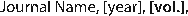
\includegraphics{head_foot/RF}}
\fancyfoot[CE]{\vspace{-7.2pt}\hspace{-14.2cm}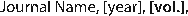
\includegraphics{head_foot/RF}}
\fancyfoot[RO]{\footnotesize{\sffamily{1--\pageref{LastPage} ~\textbar  \hspace{2pt}\thepage}}}
\fancyfoot[LE]{\footnotesize{\sffamily{\thepage~\textbar\hspace{3.45cm} 1--\pageref{LastPage}}}}
\fancyhead{}
\renewcommand{\headrulewidth}{0pt} 
\renewcommand{\footrulewidth}{0pt}
\setlength{\arrayrulewidth}{1pt}
\setlength{\columnsep}{6.5mm}
\setlength\bibsep{1pt}
%%%END OF FOOTER%%%

%%%FIGURE SETUP - please do not change any commands within this section%%%
\makeatletter 
\newlength{\figrulesep} 
\setlength{\figrulesep}{0.5\textfloatsep} 

\newcommand{\topfigrule}{\vspace*{-1pt}% 
\noindent{\color{cream}\rule[-\figrulesep]{\columnwidth}{1.5pt}} }

\newcommand{\botfigrule}{\vspace*{-2pt}% 
\noindent{\color{cream}\rule[\figrulesep]{\columnwidth}{1.5pt}} }

\newcommand{\dblfigrule}{\vspace*{-1pt}% 
\noindent{\color{cream}\rule[-\figrulesep]{\textwidth}{1.5pt}} }

\makeatother
%%%END OF FIGURE SETUP%%%

%%%TITLE, AUTHORS AND ABSTRACT%%%
\twocolumn[
  \begin{@twocolumnfalse}
{
\includegraphics[height=30pt]{head_foot/SM}\hfill\raisebox{0pt}[0pt][0pt]{
\includegraphics[height=55pt]{head_foot/RSC_LOGO_CMYK}}\\[1ex]

\includegraphics[width=18.5cm]{head_foot/header_bar}}\par
\vspace{1em}
\sffamily
\begin{tabular}{m{4.5cm} p{13.5cm} }


\includegraphics{head_foot/DOI} & \noindent\LARGE{\textbf{Instabilities of ring-rivulets: Impact of wettability patterns$^\dag$}} \\%Article title goes here instead of the text "This is the title"
\vspace{0.3cm} & \vspace{0.3cm} \\

 & \noindent\large{Stefan Zitz,\textit{$^{a\ast}$} Andrea Scagliarini,\textit{$^{b,c}$} Johan Roenby\textit{$^{a}$}} \\%Author names go here instead of "Full name", etc.

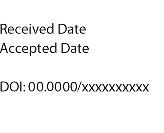
\includegraphics{head_foot/dates} & \noindent\normalsize{
\noindent Rivulets and droplets are naturally appearing shapes when small amounts of liquid are deposited on a partially wettable substrate.
Here we study, by means of numerical simulations, the dewetting dynamics of a ring-rivulet on substrates with various wettability patterns.
In particular, we consider, beyond the homogeous case, a circular-shaped patch of higher contact angle as compared to the background and a constant radial gradient of contact angle, pointing either inward or outward from the centre. We show that 
by tuning the parameters characterizing the patterns, it is possible to control 
not only the stability of the rivulet, i.e. its breakup/collapse dynamics and 
the associated time scalers, but also the dewetting morphology, in terms of number and position of the formed droplets.
%Thus making it possible to enhance the probability for a Rayleigh-Plateau type %break up into multiple droplets or to accelerate the capillary retraction that %stems from the curvature difference of the ring and leads to a single droplet.
}

\end{tabular}

 \end{@twocolumnfalse} \vspace{0.6cm}

]
%%%END OF TITLE, AUTHORS AND ABSTRACT%%%

%%%FONT SETUP - please do not change any commands within this section
\renewcommand*\rmdefault{bch}\normalfont\upshape
\rmfamily
\section*{}
\vspace{-1cm}


%%%FOOTNOTES%%%

\footnotetext{\textit{$^{a}$~IMFUFA, Department of Science and Environment, Roskilde University, Postbox 260, 4000 Roskilde, DK. Tel: +45 2993 1923; E-mail: johan@ruc.dk}}
\footnotetext{\textit{$^{\ast}$~current E-mail: stefan.zitz@rcpe.at}}

\footnotetext{\textit{$^{b}$~Institute for Applied Mathematics "M. Picone" (IAC), Consiglio Nazionale delle Ricerche (CNR), Via dei Taurini 19, 00185 Rome, Italy, E-mail: andrea.scagliarini@cnr.it}}
\footnotetext{\textit{$^{c}$~INFN, sezione Roma ``Tor Vergata'', via della Ricerca Scientifica 1, 00133 Rome, Italy}}


%Please use \dag to cite the ESI in the main text of the article.
%If you article does not have ESI please remove the the \dag symbol from the title and the footnotetext below.
\footnotetext{\dag~Electronic Supplementary Information (ESI) available: \href{https://github.com/Zitzeronion/Ring_rivulets}{Ring\_rivulets}. See DOI: 10.1039/cXsm00000x/}
%additional addresses can be cited as above using the lower-case letters, c, d, e... If all authors are from the same address, no letter is required

%\footnotetext{\ddag~Additional footnotes to the title and authors can be included \textit{e.g.}\ `Present address:' or `These authors contributed equally to this work' as above using the symbols: \ddag, \textsection, and \P. Please place the appropriate symbol next to the author's name and include a \texttt{\textbackslash footnotetext} entry in the the correct place in the list.}


%%%END OF FOOTNOTES%%%

%%%MAIN TEXT%%%%
\section{Introduction}
\label{sec:intro}
Thin liquid films and droplets are widespread in our every day life and play a crucial role
in a host of natural and technological applications, from painting and coating to lab-on-a-chip devices to biofluidics~\cite{degennesCapillarityWettingPhenomena2004, ronsinPhaseFieldSimulationsMorphology2022,fockeLabonaFoilMicrofluidicsThin2010}.
Understanding their dynamics and controlling their stability is, therefore, a central problem for applied research in process engineering and nanotechnology~\cite{singhInkjetPrintingProcess2010, quereFluidCoatingFiber1999, utadaDrippingJettingDrops2007}, but also poses fundamental questions lying at the crossroads between fluid dynamics and chemical physics~\cite{oronLongscaleEvolutionThin1997, beckerComplexDewettingScenarios2003, thielePatternedDepositionMoving2014, wilczekSlidingDropsEnsemble2017, peschkaSignaturesSlipDewetting2019}.
Dewetting induced by intrinsic instabilities of the film and/or impurities on 
the substrate surface, for instance, can undermine the effectiveness of a coating process
~\cite{bonnWettingSpreading2009, chenWrinklingInstabilitiesPolymer2012}. 
On the other hand, breakup of deposited structures such as rivulets is exploited
in the generation of droplets {\it on demand}~\cite{}.
All these phenomena involve inherently multiscale problems, that span from the molecular motion at the three phase contact line to the nano-/mircoscale thickness of the film up to the macroscopic area the coating covers, thus posing not trivial computational challenges.
The dewetting of a fluid rivulet deposited on a substrate recalls the classical fluid dynamic 
problem of a filament breakup, driven by the Rayleigh-Plateau instability, with the additional 
complexity of the fluid-solid physico-chemical interactions~\cite{diezBreakupFluidRivulets2009, diezStabilityFinitelengthRivulet2009, diezInstabilityTransverseLiquid2012}.
Recently,  a number of experimental and theoretical/numerical studies have focused on ring-shaped 
rivulets, that were shown to be useful precursors of droplet patterns with a circular symmetry~\cite{nguyenCompetitionCollapseBreakup2012, gonzalezStabilityLiquidRing2013, wuCompetingLiquidPhase2011, edwardsControllingBreakupToroidal2021}. Here, at difference with the simpler
straight rivulet case, the dewetting dynamics depends also on the non-uniform curvature of the rivulet ringed shape,
and in particular on the different curvatures of the two contact lines.
%Recently, Suo et al.~\cite{suoDewettingCornerFilm2023} have studied a related problem where the film admits a %wedge shape and a solid cylinder fills the inner part of the ring. 
%The ring is therefore not allowed to contract, but can breakup and form droplets.
%They further show a good agreement between theory and simulations as well as a clear dependence of the %dynamics on the initial width of the film and the contact angles at each boundary.
Self- and direct assembly of nanomaterials from liquid nanostructures has been one of the driving forces for the study of Nguyen et al.~\cite{nguyenCompetitionCollapseBreakup2012} and earlier studies of Wu et al.~\cite{wuBreakupPatternedNanoscale2010} where they showed that liquid-metal rings are suited to form arrays of droplets.
Diez et al.~\cite{diezBreakupFluidRivulets2009, diezStabilityFinitelengthRivulet2009} laid the theoretical foundation for the stability of a straight rivulet in their work using linear stability analysis (LSA) and numerical simulations. 
Later, Gonz{\'a}lez et al.~\cite{gonzalezStabilityLiquidRing2013} extended these results to ring rivulets, determining the characteristic time scales for collapse and breakup and showing that the main control parameter
discriminating between the two instability routes is the rivulet aspect-ratio, namely the ratio of its 
width over the its radius.
They also provided predictions on the expected number 
of formed droplets as dictated by the most unstable wavelength.
An interesting question that may naturally arise is whether and to which extent it is possible to further 
control the fate of ring rivulets and the consequent dewetting morphologies by properly treating the substrate
to exploit wettability patterns 
With recent developments in surface chemistry and the emerging technology of switchable substrates
local precise wettability gradients are now attainable more than ever~\cite{xinReversiblySwitchableWettability2010, stuartEmergingApplicationsStimuliresponsive2010,chenThermalresponsiveHydrogelSurface2010, ichimuraLightDrivenMotionLiquids2000, mugeleElectrowettingConvenientWay2005, edwardsControllingBreakupToroidal2021} .
While a number of studies have focused on thin film dewetting and droplet transport on patterned substrates~\cite{liuActuatingWaterDroplets2015,grawitterSteeringDropletsSubstrates2021, zitzControllingDewettingMorphologies2023}, the case of ring-shaped rivulets remained so far almost unexplored.
A relevant exception is represented by the work of Edwards et al~\cite{edwardsControllingBreakupToroidal2021},
who have studied numerically and experimentally liquid rings deposited on substrate whose contact angle 
was controlled by electrowetting. They showed that different electric potentials can be used not only to control the number of droplets after breakup but also to fully reverse the process.
In this paper, we present a systematic study of the effect of the ring rivulet initial geometry (width over 
radius ratio) and of two types of wettability patterns in the 
selection of route towards either retraction and collapse to a single droplet or towards the breakup into multiple 
droplets. We show that by depositing the liquid ring onto an annular region of lower contact angle (with respect to the background substrate) one can remove the collapse mode and, moreover, the contact angle 
contrast turns out to be a further means of control, together with the dimensionless initial ring width,
on the number of droplets at equilibrium.
By introducing, instead, a radially symmetric linear contact angle profile, coaxial with the ring and pointing either inwards or outwards, we find that it is possible, in the former case, to control the retraction speed 
while steering the number of metastable droplets whereas, in the latter case, to stabilize the ring rivulet 
against collapse.
The outline of the paper is as follows: In the next section, Sec.~\ref{sec:method} we introduce the method we use to run numerical experiments.
We then present our results in Sec.~\ref{sec:dynamics}, starting with a comparison with the literature and then present the impact of the wettability patterns.
In the last section, Sec.~\ref{sec:conclu} we give a short summary, highlighting important results and conclude with an outlook of possible research applications.

\section{Simulation method}
\label{sec:method}
%For the time resolved simulations of a thin liquid ring-rivulet we use a recently developed lattice Boltzmann %method (LBM)~\cite{zitzLatticeBoltzmannMethod2019, zitzLatticeBoltzmannSimulations2021, zitzSwalbeJlLattice2022, %zitzControllingDewettingMorphologies2023}. 
We perform numerical simulations of the thin film equation (TFE),  
\begin{equation}\label{eq:thinsolve}
     \partial_t h(\mathbf{x},t) = \nabla\cdot\left(M_{\delta}(h)\nabla p\right),
\end{equation}
where $\mathbf{x} = (x,y)$ and $\nabla = (\partial_x, \partial_y)$, by means of a recently 
developed lattice Boltzmann method~\cite{zitzLatticeBoltzmannMethod2019, zitzLatticeBoltzmannSimulations2021, zitzSwalbeJlLattice2022, zitzControllingDewettingMorphologies2023}. 
The mobility function $M_{\delta}(h) = \frac{h^2}{\mu\alpha_{\delta}(h)}$ with 
\begin{equation}\label{eq:alphafric}
    \alpha_{\delta}(h) = \frac{6h}{(2 h^2 + 6 \delta h + 3 \delta^2)},
\end{equation}
which for the no-slip boundary condition $(\delta \rightarrow 0)$ becomes $M_{0}(h) = h^3/3\mu$, where $\delta$ is an effective slip length and $\mu$ is the dynamic viscosity, both values can be found in App.~\ref{app:numerics}.
We like to point out, however, that the slip length value is within the weak/intermediate slip regime~\cite{peschkaSignaturesSlipDewetting2019,fetzerQuantifyingHydrodynamicSlip2007, munchLubricationModelsSmall2005} and has been used in previous work~\cite{zitzControllingDewettingMorphologies2023}.
The pressure $p$ in Eq.~(\ref{eq:thinsolve}) is given by,
\begin{equation}\label{eq:filmpressure}
    p = - \gamma\nabla^2 h -\Pi(h),
\end{equation}
with $\Delta h$ being the 2D Laplacian of the liquid-gas interface and $\Pi(h)$ is a so-called disjoining pressure~\cite{schwartzSimulationDropletMotion1998, crasterDynamicsStabilityThin2009, nguyenCompetitionCollapseBreakup2012, gonzalezStabilityLiquidRing2013}
\begin{equation}\label{eq:disjoinpressure}
    \Pi(h,\theta) = \frac{2\gamma}{h_{\ast}}[1-\cos\theta(\mathbf{x})]\left[\left(\frac{h_*}{h}\right)^3 -\left(\frac{h_*}{h}\right)^2\right],
\end{equation}
where $\gamma$ is the surface tension, $h_{\ast}$ is a precursor thickness, see App.~\ref{app:numerics}, at which $\Pi(h_{\ast}, \theta) = 0$ and $\theta$ is an equilibrium contact angle.
By varying $\theta$ in Eq.~(\ref{eq:disjoinpressure}) we have an effective model for a patterned substrate, see e.g., Refs~\cite{zitzLatticeBoltzmannSimulations2021, zitzControllingDewettingMorphologies2023}. 
The contact angle, in agreement with the lubrication approximation~\cite{oronLongscaleEvolutionThin1997, crasterDynamicsStabilityThin2009}, is set within the bounds $[\pi/18, 2\pi/9]$, except for the banded pattern, see Sec.~\ref{subsubsec:banded}. 
%Our strategy is therefore to iterate Eq.~(\ref{eq:thinsolve}) in time and let the rivulet find a stable %configuration, with some upper limit on simulation time as discussed in App.~\ref{app:numerics}.
%This stable configuration can either be several disconnected droplets if the rivulet breaks up or a single %coalleased droplet in the middle of the domain.  

\subsection{Initial conditions}
\begin{figure}
\centering
  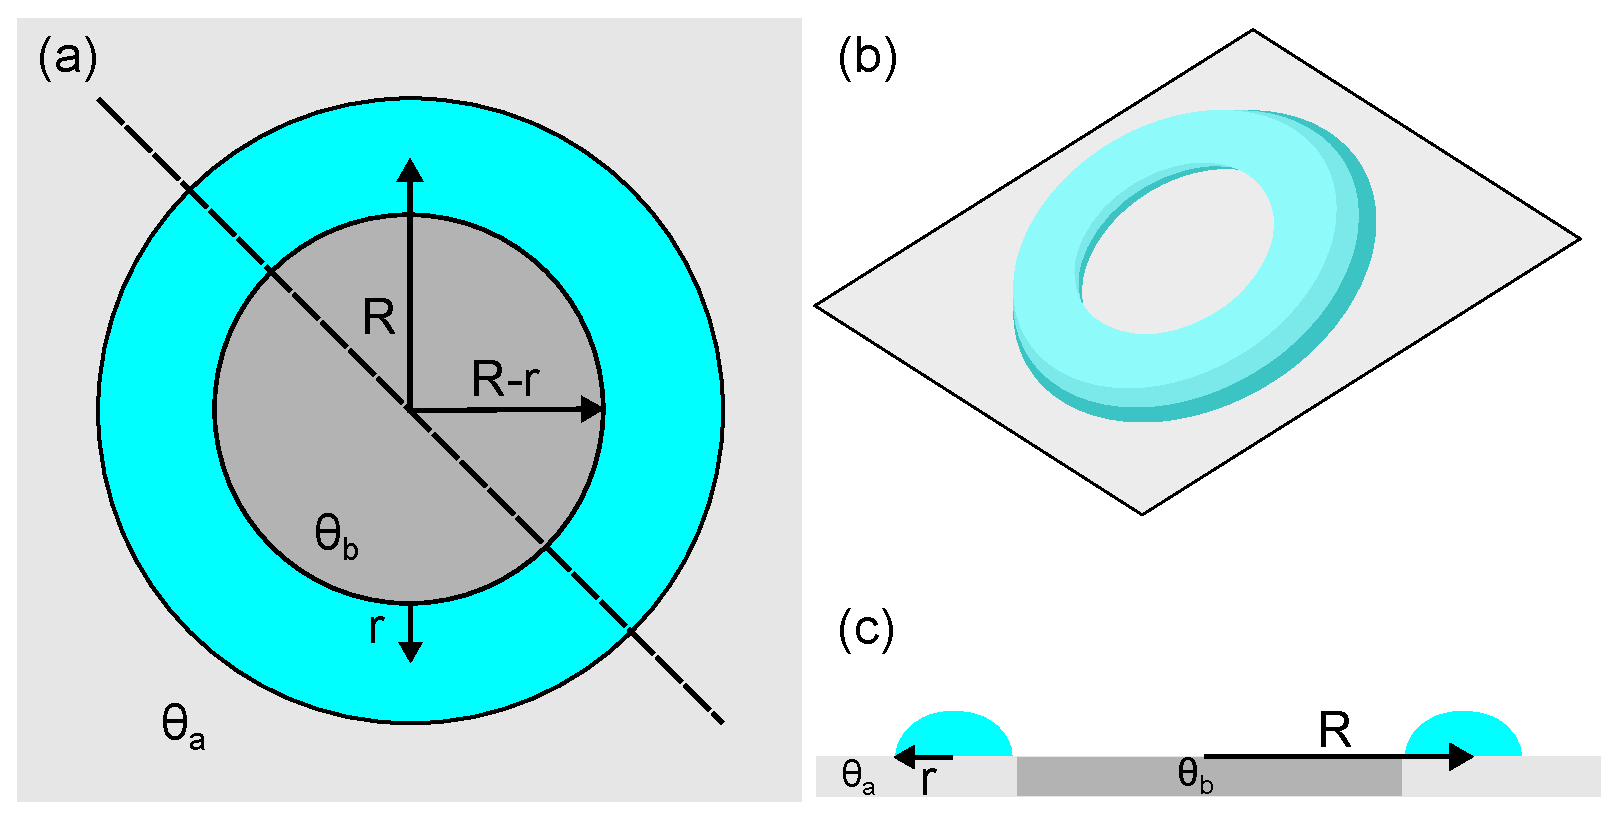
\includegraphics[width=0.45\textwidth]{ringrivulet_shema}
  \caption{Schematic setup of our initial conditions. In (a) we show the top view where $R$ and $r$ are the two different radii and $\theta_a$ and $\theta_b$ can be different contact angles. 
  In (b) we show an isometric view of the initial condition.
  By cutting along the dashed line in (a) we get the side view of (c).}
  \label{fig:ringschema}
\end{figure}

We initialise the thickness profile $h_0(\mathbf{x})=h(\mathbf{x}, t=0)$ by first imposing the shape of a toroidal cap, with radial symmetry along the $z$-axis, centred in the origin of the coordinate system
and with major an minor radii $R_0$ and $r_0$,
whose equation in polar coordinates $(\xi, \phi)$ (with $x = \xi \cos(\phi)$, $y=\xi \sin(\phi)$ reads,
% \begin{strip}
\begin{equation}\label{eq:torus}
h_0(\mathbf{x})=\left(\sqrt{r_0^2 - \left(R_0-\xi\right)^2} - r_0\cos \theta_0 + h_{\ast}\right)
\end{equation}
for $|R_0-\xi|<r_0 \sin \theta_0$ (and $h_0(\mathbf{x})=h_{\ast}$, otherwise); then, we let it relax to the actual 
equilibrium shape~\cite{diezBreakupFluidRivulets2009} which we slightly perturb with a Gaussian noise with zero mean and variance $10^{-4}r_0^2 \sin^2\theta_0$. 
%\begin{equation}\label{eq:torus}
%h_0(\mathbf{x}) = 
%\left\{
%\begin{array}{ll}
%\left(B - r_0\cos(\theta) + h_{\ast}\right)(1+\varepsilon\mathcal{N})  & \mbox{if } |R_0-\xi|<r_0 %\sin(\theta)\\
%h_{\ast} & \mbox{otherwise}
%\end{array}
%\right.
%\end{equation}
% \end{strip}
%where $B = \sqrt{r_0^2 - \left(R_0-\xi\right)^2}$, $R_0$ and $r_0$ are the major and minor torus radii, respectively (see Fig.~\ref{fig:ringschema}).
%$\mathcal{N}$ is a Gaussian random variable with zero mean and 
%unit variance and  $\varepsilon = 10^{-2}$.

\section{Results}
\label{sec:dynamics}
\begin{figure*}
    \centering
    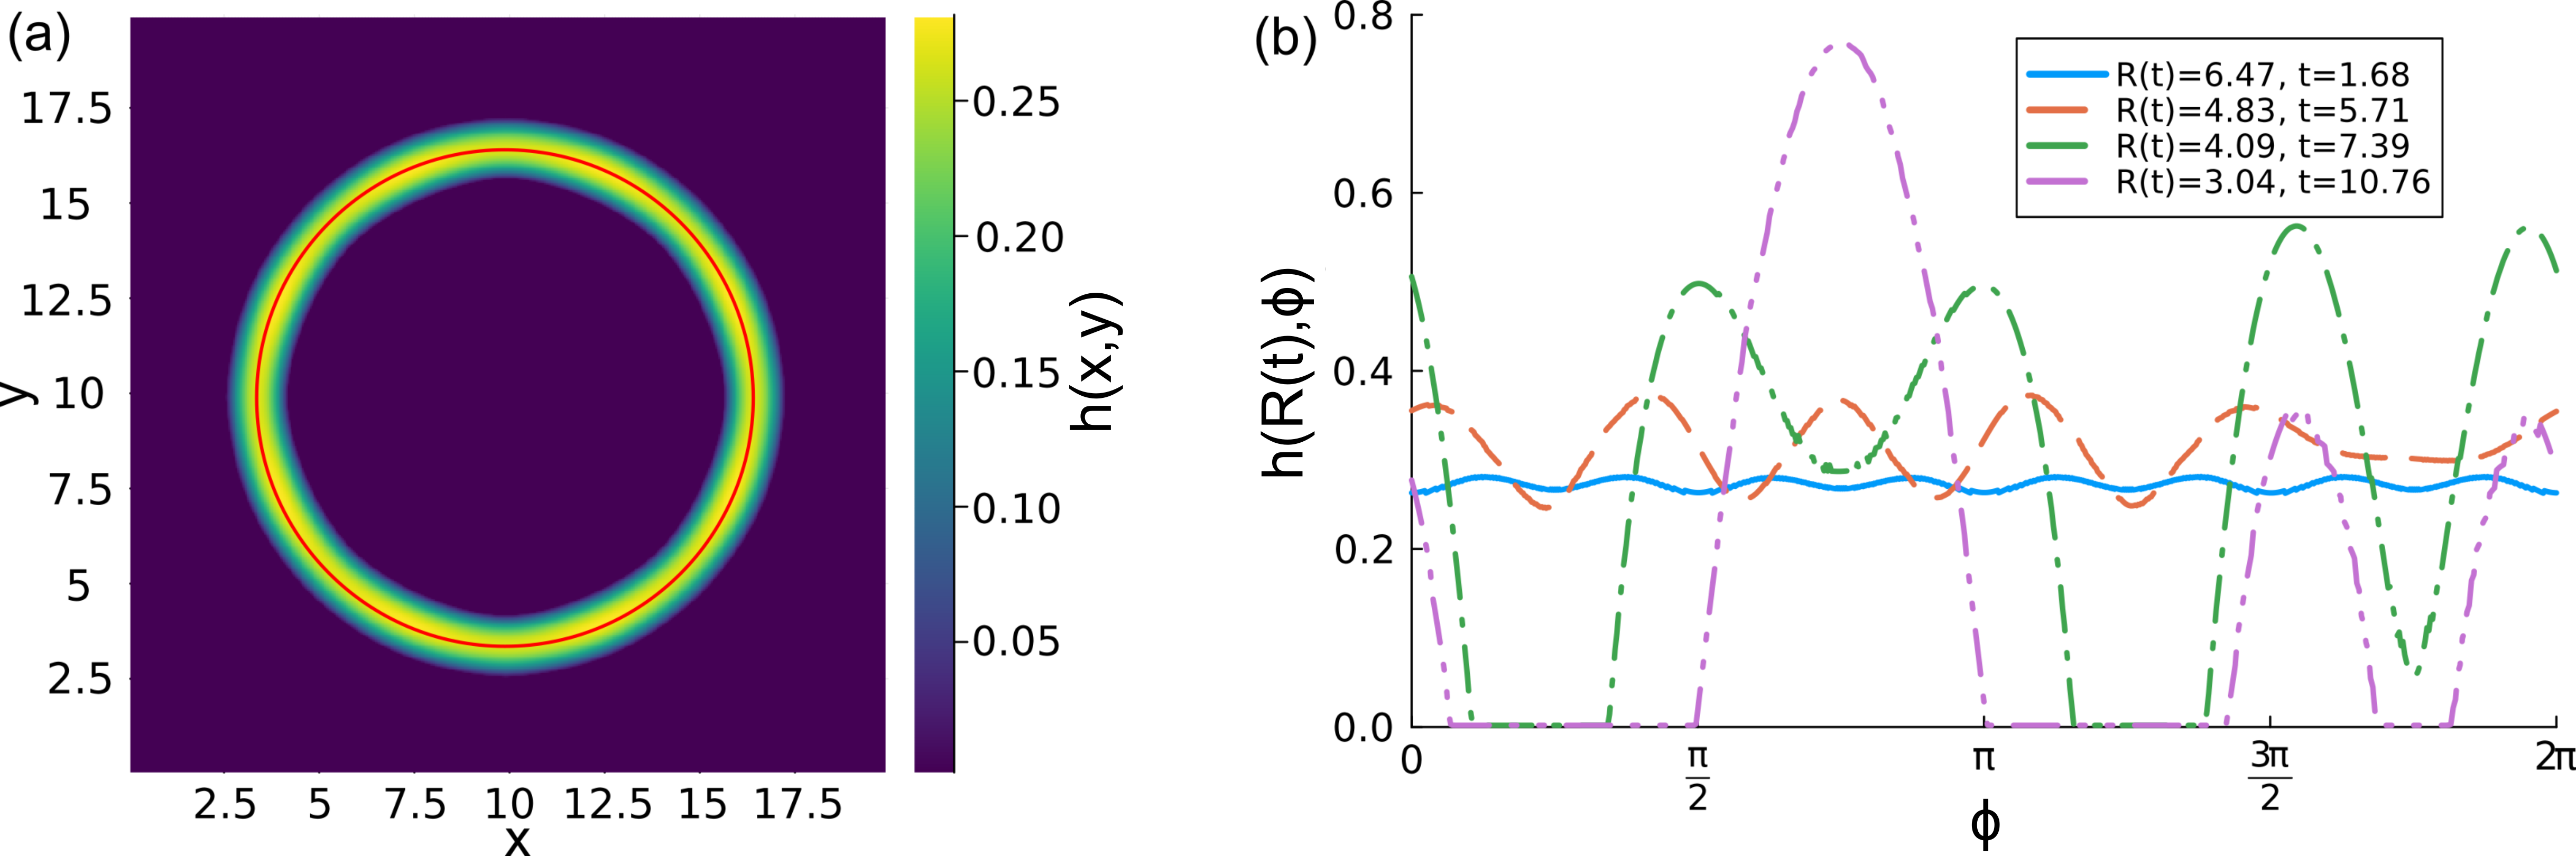
\includegraphics[width=0.95\textwidth]{assets/heatcirc_2.png}
    \caption{(a) Heatmap of the film thickness at $t=1.68\tau_m$ for $\psi_0 = 0.21$. 
    All length scales are normalized by $H_D = 25.67$. 
    The red ring in the middle of the rivulet is depicted as blue line plot in (b).
    In (b) we show circular profiles of the film thickness, $h(\xi=R(t),\phi,t)$, for different time steps.
    The dynamics initially selects an unstable mode with wavelength $\lambda \approx (2 \pi R_0)/8$, 
    but as the ring srinks, eventually it breaks up into only $3$ droplets, corresponding to the three maxima of the purple curve.}
    \label{fig:ThreeDToOneD}
\end{figure*}

\subsection{Instability paths}\label{subsec:stability}

Following Gonz\'alez et al~\cite{gonzalezStabilityLiquidRing2013} we introduce the dimensionless width
parameter, or aspect-ratio, defined as the ratio of the initial rivulet width over radius, 
$\psi_0 \equiv 2r_0 \sin(\theta_0)/R_0$. It was shown numerically and proved theoretically~\cite{gonzalezStabilityLiquidRing2013,nguyenCompetitionCollapseBreakup2012}
 that if $\psi_0$ is large enough, rectractive collapse takes place, otherwise the rivulet tends to breakup 
 and form droplets.

%In previous studies~\cite{gonzalezStabilityLiquidRing2013} the focus %was set on the three-phase contact lines and the LSA predictions %agreed well with the slip model simulations.
%Among the many results of this work is the fact that the varicose %modes are always growing stronger than the zigzag modes.
%The stability, then, is associated with the width of the ring-%rivulet $w = 2r$ as well as the ratio of radii $\psi_0 = 2r/R_0 = w/%R_0$ 
%When the width approaches zero, $w \rightarrow 0$, the rivulet %breaks up and is likely to form independent droplets.

In order to have a quantitative insight on the ring rivulet evolution we track the growth of the following 
observable:
\begin{equation}\label{eq:delta-h-measure}
       \Delta h(t) = \max_{\phi}h(R(t),\phi,t) - \min_{\phi}h(R(t),\phi,t),
\end{equation}
where $R(t) = (r_i(t)+r_o(t))/2$ and $r_{i,o}(t)$ indicate the location of the inner and outer contact lines, 
respectively. 
%which can be computed from Fig.~\ref{fig:ThreeDToOneD}(b).
%This measure has the advantage that it is well within the rivulet and thus should %filter out a constant background from the precursor film $h_{\ast}$, see %Eq.~(\ref{eq:disjoinpressure}).

\begin{figure}
    \centering
    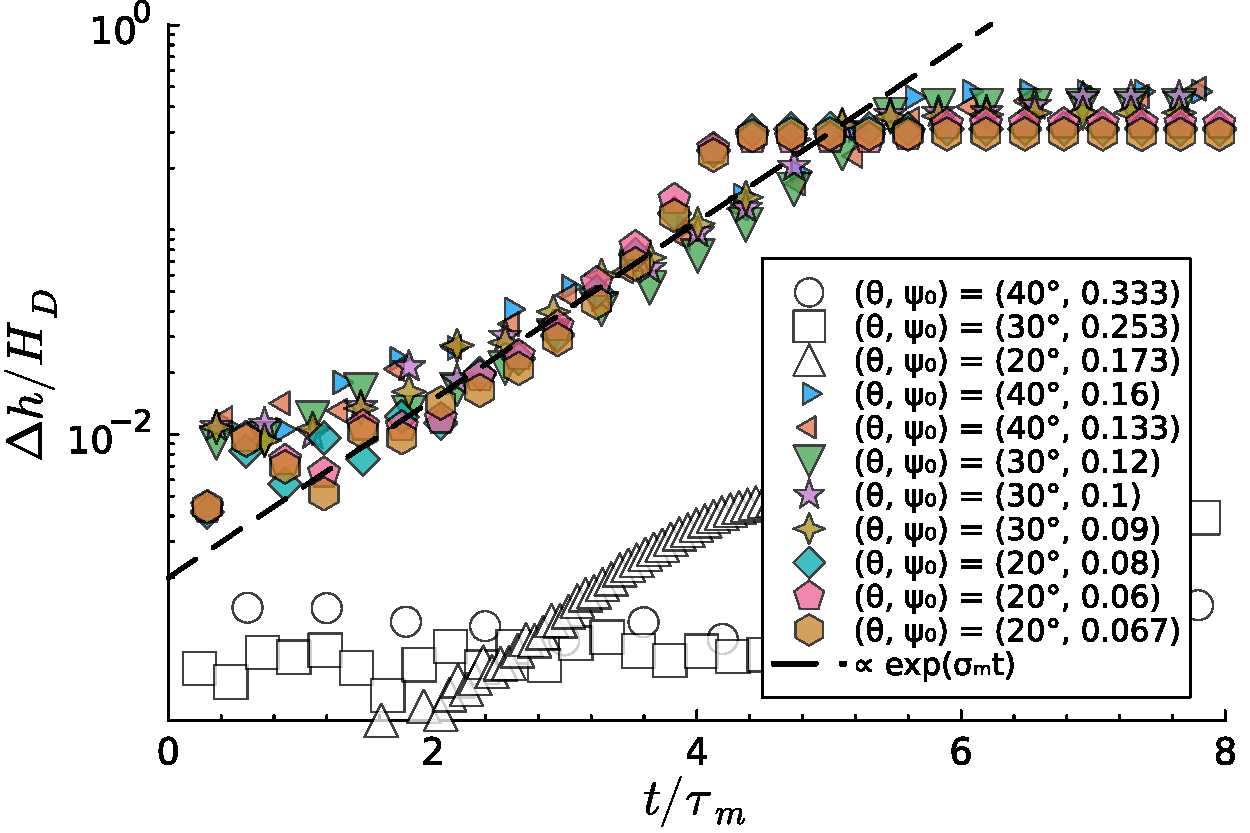
\includegraphics[width=0.45\textwidth]{assets/growth-breakup.pdf}
    \caption{Thickness difference $\Delta h$ normalized by the height of a spherical cap droplet that contains all liquid $H_D$ along the curve at radius $\xi(h_{\max})$ over time normalized by $\tau_m \propto (\mu R/\gamma) \sin(\theta_0)/\theta_0^{3/2}$ for the uniform pattern. 
    Different symbols depict different initial conditions. 
    Full or empty symbols distinguish between breakup and collapse. 
    The black dashed curve shows an exponential growth $e^{t/\tau_m}$, see Eq.~(\ref{eq:growth-sigma}).
    }
    \label{fig:first_growth}
\end{figure}
%As a criterion for a breakup we assume 
%$\Delta h(\tau_b) \approx 2r(1-\cos(\theta)$.
Such quantity should grow exponentially in the linear instability regime~\cite{wuBreakupPatternedNanoscale2010, gonzalezStabilityLiquidRing2013, nguyenCompetitionCollapseBreakup2012}, with a growth rate that depends on 
both the aspect-ratio $\psi_0$ and on the contact angle $\theta_0$~\cite{gonzalezStabilityLiquidRing2013}; for $\psi_0 \ll 1$, though, the dynamics approximates the 
linear rivulet case and the growth is essentially independent on $\psi_0$. In fact, in this limit, 
as shown with full symbols in Fig.~\ref{fig:first_growth}, we could achieve a nice collapse of the $\Delta h$ vs $t$ 
curves for different couples $(\theta_0,\psi_0)$, provided the time is rescaled by the characteristic, contact angle dependent, time 
$\tau_m \propto (\mu R/\gamma) \sin(\theta_0)/\theta_0^{3/2}$. 
The rescaling, on the contrary, does not work for large $\psi_0$ (empty symbols in Fig.~\ref{fig:first_growth}), when ring collapse takes place, leading to the closure of the inner hole 
and to the formation of single droplet.

\subsection{Dewetting on uniform substrates}\label{subsec:drop-counting}

We start our analysis of the dewetting dynamics of a ring-rivulet considering substrates with uniform wettability (i.e. constant contact angle 
$\theta(\mathbf{x}) = \theta_0$). In order to discriminate between the two 
available dewetting paths, we look at the final number of droplets $n_d$, which 
the ring-rivulet ends up into, as a function of $\psi_0$.
\begin{figure}
    \centering
    %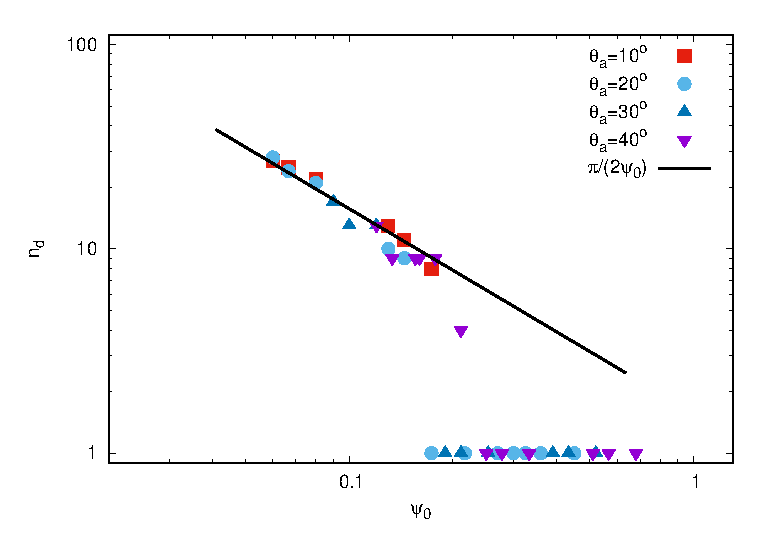
\includegraphics[width=0.45\textwidth]{n_drops_vs_psi_uniform.eps}
    %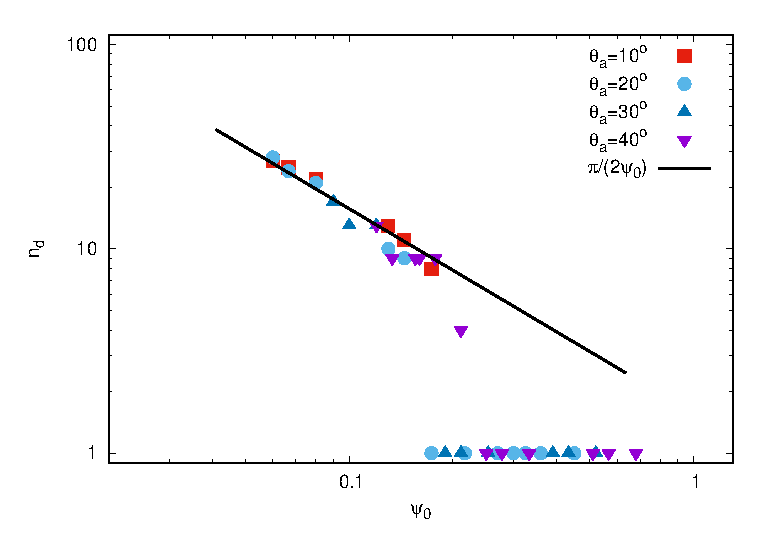
\includegraphics[width=0.45\textwidth]{n_drops_vs_psi_uniform.eps}
    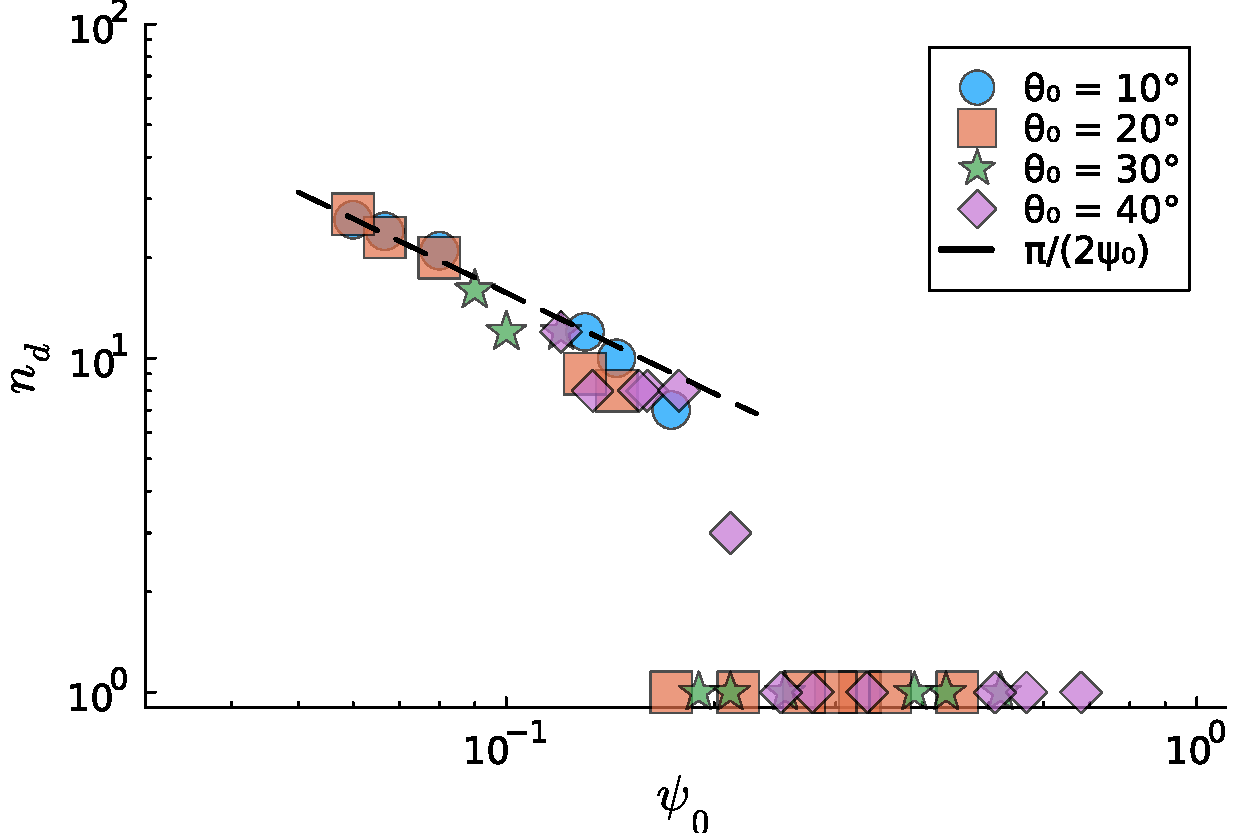
\includegraphics[width=0.45\textwidth]{assets/Ndrops_uni_new.pdf}   
    \caption{Droplet number $n_d$ vs aspect ratio $\psi_0$ on uniform substrates 
    for various contact angles $\theta_0$. The solid line depicts the 
    approximated LSA prediction, Eq.~(\ref{eq:maxDrops})~\cite{gonzalezStabilityLiquidRing2013}.}
    \label{fig:max_drops}
\end{figure}
We see from Fig.~\ref{fig:max_drops}, where we report $n_d$ vs $\psi_0$
for various contact angles, that for small aspect-ratio, $\psi_0 <0.2$,
$n_d>1$, indicating that the rivulet undergoes a breakup, whereas for $\psi_0>0.2$ 
we get $n_d=1$, signalling the retractive collapse to a single droplet located in the centre of the domain.
When breakup takes place, moreover, we observe that $n_d$ decreases with $\psi_0$ in agreement with the approximated formula 
\begin{equation}\label{eq:maxDrops}
    n_d \approx \frac{\pi}{2\psi_0},
\end{equation}
(solid line in Fig.~\ref{fig:max_drops}) 
derived from linear stability analysis (LSA) assuming that 
the most unstable mode determines the number of droplets~\cite{gonzalezStabilityLiquidRing2013}.
The agreement is particularly good for small contact angles, as it should be expected since the theory that leads to (\ref{eq:maxDrops}) does not account for the disjoining pressure~\cite{gonzalezStabilityLiquidRing2013}. Interestingly, as the contact angle increases
the number of droplets becomes almost independent of $\psi_0$, suggesting that the 
breakup process is mainly driven by the reduced wettability of the substrate.
%However, Gonz{\'a}lez et al.~\cite{gonzalezStabilityLiquidRing2013} pointed out that the LSA and thus $n_{\max}$ fall short if one considers a disjoining pressure model, see Eq.~(\ref{eq:disjoinpressure}).
%They report that although initially the rivulet adapts to its most unstable mode it does not necessary break up into $n_{\max}$ droplets, especially for $\psi_0 > 0.15$. 
%They also point towards the experiments of Wu et al.~\cite{wuCompetingLiquidPhase2011} where a similar mismatch with theoretical predictions was observed.

%We perform a similar analysis and count the number of droplets during our numerical experiments and adopted the scheme introduced by Gonz{\'a}lez et al.~\cite{gonzalezStabilityLiquidRing2013}, thus count the collapse as zero droplets, one off center droplet as one, two droplets as two and so on.
%The result is shown in Fig.~\ref{fig:max_drops}, where the black line is given by Eq.~(\ref{eq:maxDrops}) and the different symbols refer to a uniform substrate and the band pattern Eq.~(\ref{eq:theta_band}).
% Our results tend to agree with the observations made by Gonz{\'a}lez et al.~\cite{gonzalezStabilityLiquidRing2013}.
%In Fig.~\ref{fig:ThreeDToOneD} we actually observe a transition from $n = 8$ (blue curve) to $n = 3$ (purple curve), observing only three droplets after breakup.

% We can further quantify this behavior in terms of time scales for both the collapse and the breakup of the ring-rivulet.
%In Fig.~\ref{fig:max_drops} we see that for larger $\psi_0$-values theory and our numerical experiments do not match.
%In fact, for $\psi_0 > 0.2$ the ring-rivulet on the homogeneous substrate (\textcolor{jlorange}{$\star$}) favours the collapse $n = 0$. 
%It is therefore fair to assumes that the growth-rate of the instability is slower than the rate of collapse, thus $t_b > t_c$ for $\psi_0 > 0.22$, see Fig.~\ref{fig:first_growth} empty symbols.
%%%%%%%%%%%%%%%%%%%%
Taking $\psi_0 \approx 0.2$, at which $n_d$ drops to one, then, as the 
value discriminating between breakup and collapse, we now focus on the 
characteristic times of both processes.
In Fig.~\ref{fig:timescaleDifference} we report the breakup (top panel) 
collapse times (bottom panel) as a function of $\psi_0$.
Hereafter times are made dimensionless by a characteristic capillary time $t_c$, defined as 
$t_c = \mu H_0/\gamma$, where $H_0=1-\cos \theta$ is the initial rivulet maximum thickness.
\begin{figure}
    \centering
    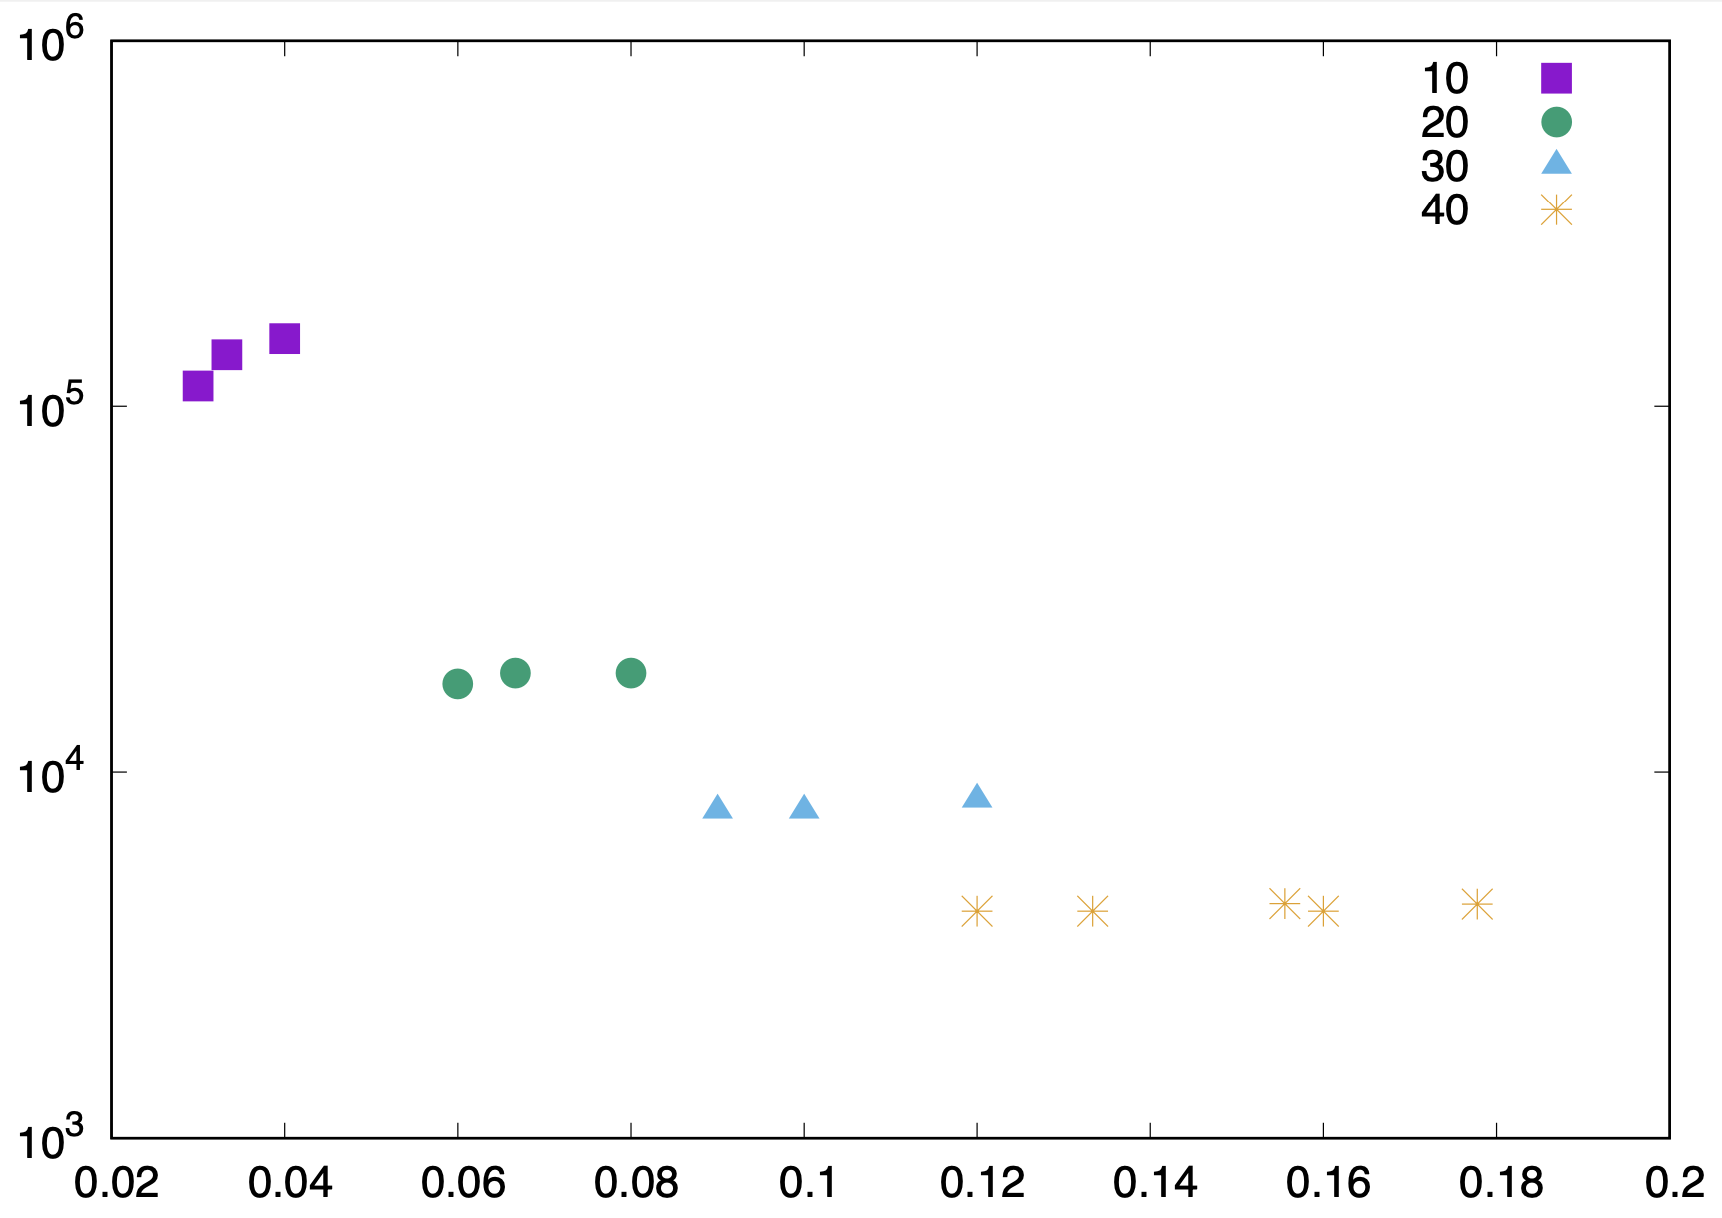
\includegraphics[width = 0.45\textwidth]{taub_vs_psi0.png}
    \caption{(Top panel). Rivulet breakup times for various substrate contact angle 
    as a function of the initial aspect-ratio $\psi_0$. (Bottom panel) Collapse times vs $\psi_0$ for various substrate contact angle. In both figures the times
    have been made dimensionless by $t_c = \mu H_0/\gamma$, 
    where $H_0=1-\cos \theta$ is the initial rivulet maximum thickness.}
    \label{fig:timescaleDifference}
\end{figure}

\subsection{Wettability patterns}\label{subsec:wettability}

We now focus on the rivulet stability and dewetting morphology on 
substrates with space-varying contact angle (i.e. {\it patterned substrates}).
As anticipated in the introduction, we consider two different wettability patterns: i) a  circular patch 
\begin{equation}\label{eq:theta_band}
    \theta(\xi) =\begin{cases}
        \theta_b,\quad \text{for}~\xi < R - r_0\sin(\theta_0) \\
        \theta_a \equiv \theta_0,\quad \text{otherwise}
    \end{cases},
\end{equation}
ii) an axially symmetric linear contact angle profile
\begin{equation}\label{eq:theta_grad}
    \theta(\xi) = \frac{\theta_{a}-\theta_{b}}{R_0} \xi + \theta_{b},
\end{equation}
where either $\theta_{a} > \theta_{b}$ (outward pointing gradient) or $\theta_a < \theta_b$ (inward pointing
 gradient).
The different contact angle patterns are then used in Eq.~(\ref{eq:disjoinpressure}) which, in turn, enters in Eq.~(\ref{eq:thinsolve}) through the total pressure, Eq.~(\ref{eq:filmpressure}).
The idea behind such choices is that the former serves as an effective boundary which removes the collapse mode and the latter helps us to understand the force balance between wetting and retraction of the ring-rivulet, see Eqs.~(\ref{eq:theta_band}-\ref{eq:theta_grad}).


\subsubsection{Circular patch}\label{subsubsec:banded}
This pattern, Eq.~(\ref{eq:theta_band}), is realized by using $\theta_a \equiv \theta_0 \in [10^{\circ}, 20^{\circ}, 30^{\circ}, 40^{\circ}]$ and $\theta_b = 60^{\circ}$, which yields a contact angle contrast $\Delta\theta \in [50^{\circ}, 40^{\circ}, 30^{\circ}, 20^{\circ}]$.
While this choice seem to contracting the long wave approximation, we actually do not see the film penetrating the $\theta_b$ region in our numerical experiments.
Thus, the substrate area $\pm\delta\xi$ away from the ring-rivulets base can be understood as an effective barrier. 
Edwards et al.~\cite{edwardsControllingBreakupToroidal2021} performed related experiments where they were able to remove the coalescence mode with elaborate surface coatings and used electrowetting to dynamically modify the contact angle.
\begin{figure}
    \centering
    %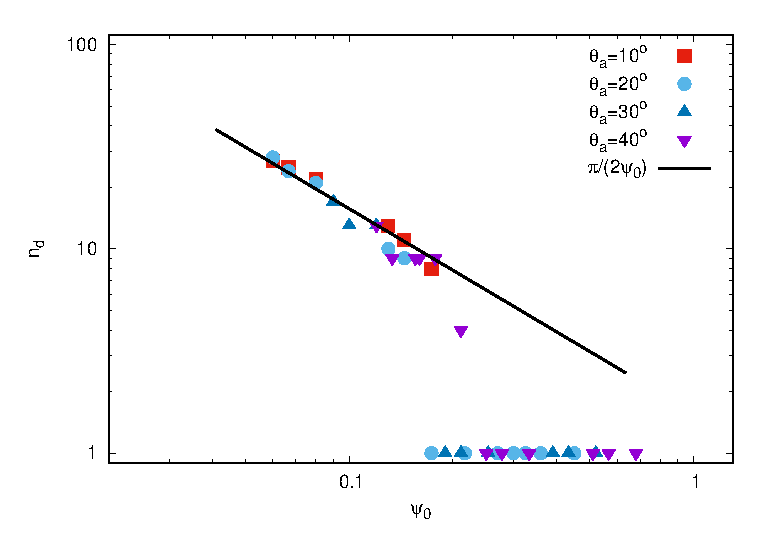
\includegraphics[width=0.45\textwidth]{n_drops_vs_psi_uniform.eps}
    %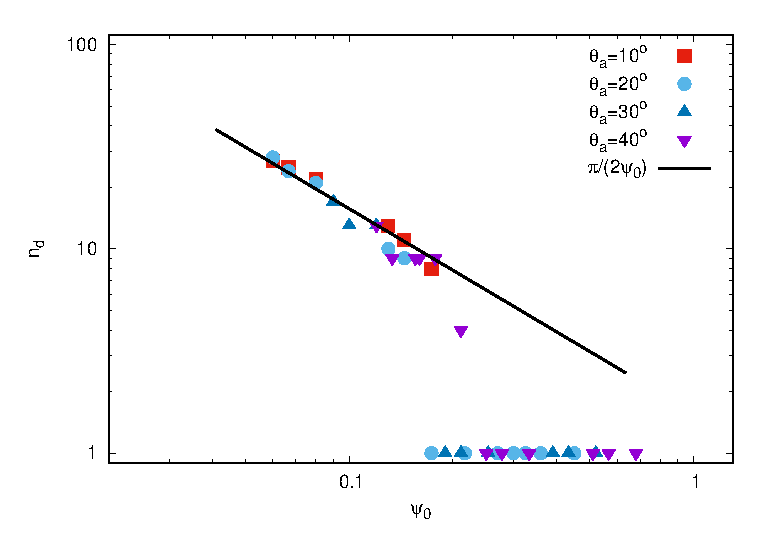
\includegraphics[width=0.45\textwidth]{n_drops_vs_psi_uniform.eps}
    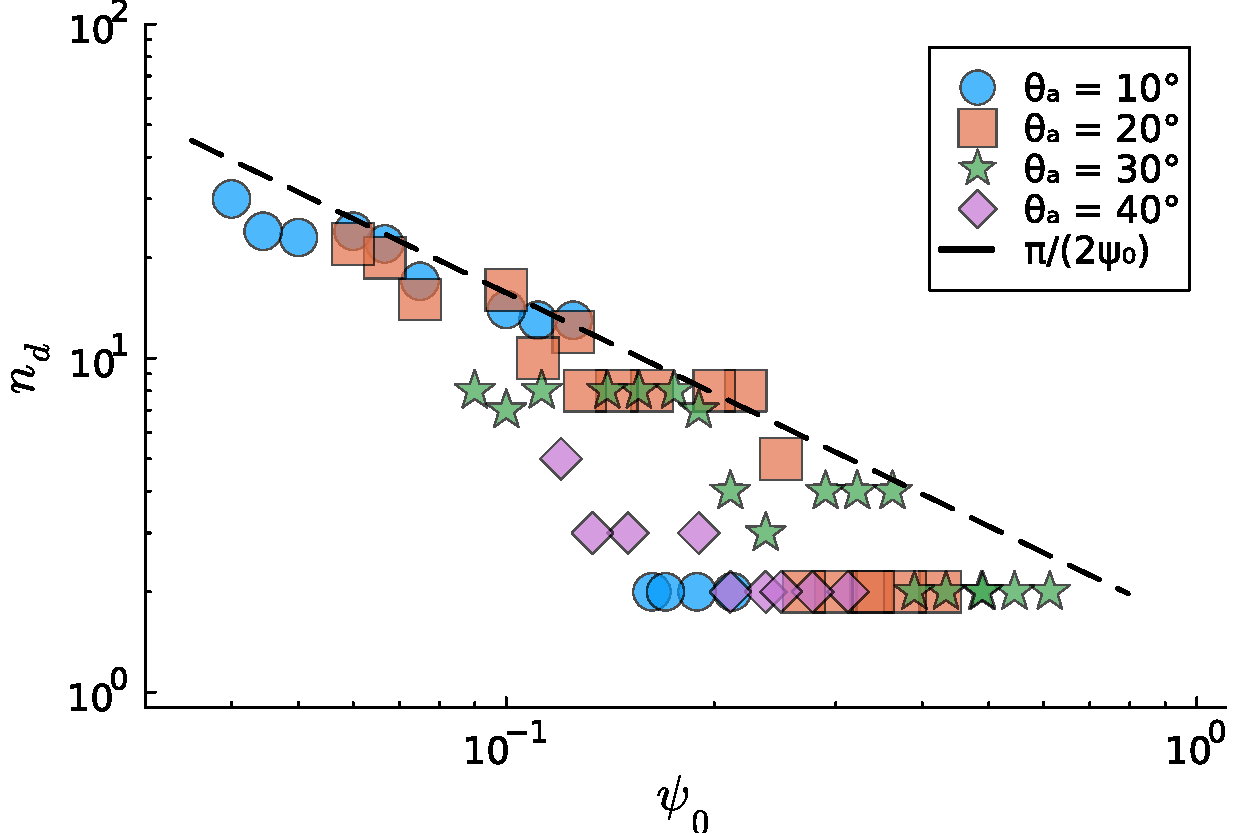
\includegraphics[width=0.45\textwidth]{assets/Ndrops_ban_new.pdf}    
    \caption{Droplet number $n_d$ vs aspect ratio $\psi_0$ on substrates patterned with 
    the circular patch, Eq.(\ref{eq:theta_band}).
    for various contact angles $\theta_0$. The solid line depicts the 
    approximated LSA prediction, Eq.~(\ref{eq:maxDrops})~\cite{gonzalezStabilityLiquidRing2013}.}
    \label{fig:max_drops}
\end{figure}
\begin{figure}
    \centering
    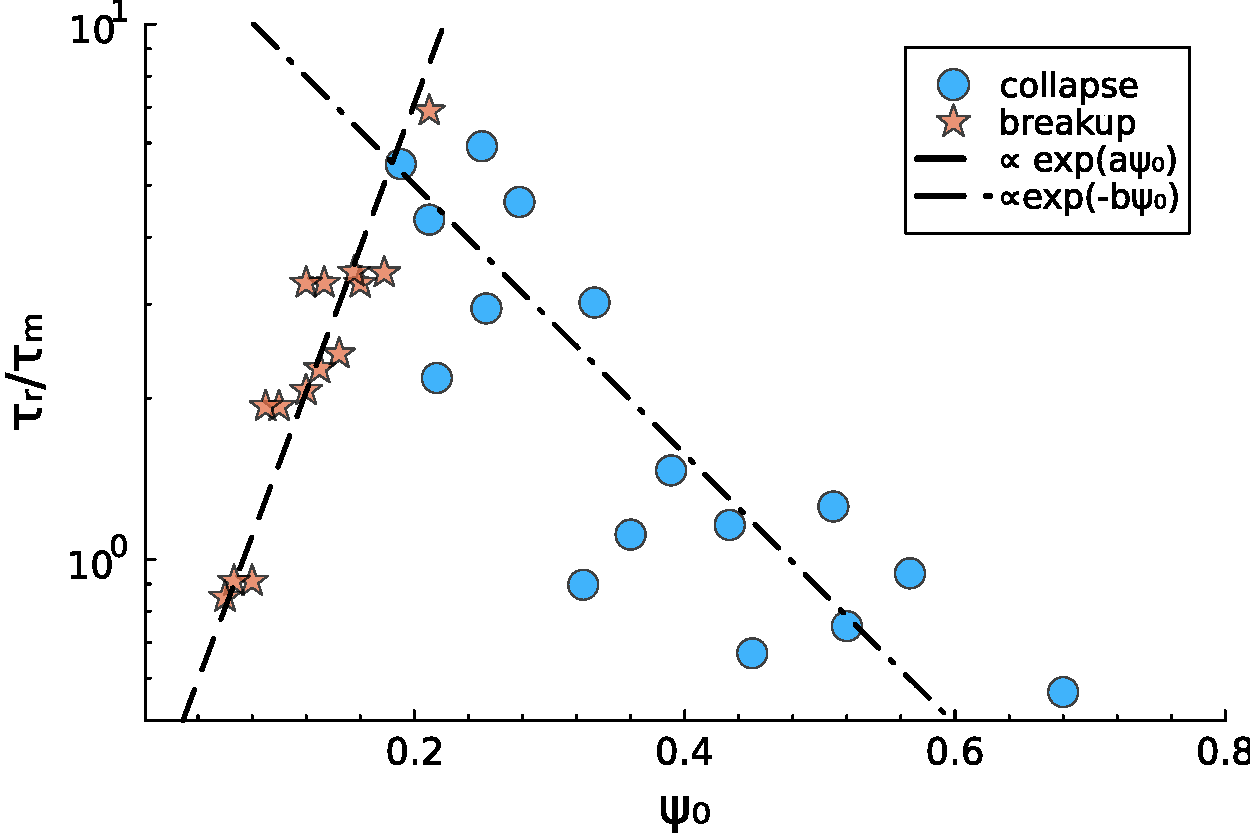
\includegraphics[width=0.48\textwidth]{assets/bandBreakup_timescales.pdf}
    \caption{Breakup times $\tau_b$ \textcolor{red}{AS: In the figure it is written $\tau_r$. Please, fix it} normalized by their respective $\tau_m$ for the banded case Eq.~\ref{eq:theta_band}.
    Different colors depict different contact angle contrasts $\Delta\theta$.
    The dashed line is a linear function of $\psi_0$. %with $La = \gamma\rho R_0/\mu^2$ as slope.
    }
    \label{fig:bandBreakupT}
\end{figure}
Because the initial configuration is unstable, the ring-rivulet will eventually rupture and form droplets, this however can be on long time scales depending on $\psi_0$.
In Fig.~\ref{fig:bandBreakupT} we measure the rupture times $\tau_b$ normalized by their respective $\tau_m$ for different initial conditions on the banded substrate.
Different colors indicate different contact angle contrasts $\Delta\theta$ and although there is not a complete collapse of the data, it seems that there is a linear trend between $\tau_b/\tau_m$ and $\psi_0$.
To highlight this statement we add a linear fit in Fig.~\ref{fig:bandBreakupT} as a black dashed line. 

Although having numerical experiments run up to $t = 25\tau_m$ we do not always observe the breakup. 
This is indicated in by the $n_{\max} = 1$ data in Fig.~\ref{fig:max_drops}, where the bullets (\textcolor{black}{$\bullet$}) show data from the banded pattern. 
In those simulations the ring-rivulet has not ruptured at the end of the simulation time.
However, $\Delta h$ measurements show growth in some cases.
% In contrast to the uniform substrate we do not see any $n_{\max} = 0$ event. 
We see that the predicted number of droplets Eq.~(\ref{eq:maxDrops}) does not fit the data as good as for the uniform substrate. 
Similarly to the uniform substrate and in agreement with previous work~\cite{gonzalezStabilityLiquidRing2013} we see similar behavior as in Fig.~\ref{fig:ThreeDToOneD}.
Thus, having $n = n_{\max}$ for early time scales but at rupture we get $n < n_{\max}$.

\subsubsection{Linear wettability gradients}\label{subsubsec:linwettgrad}
So far we have shown that our numerical experiments can, first, reproduce known results and second are able to address the aspect of wettability.
We find that a larger contact angle leads to deviations from Eq.~(\ref{eq:maxDrops}) but growthrates $\sigma_m$ can be collapsed.
Further we have shown that a pattern can be used remove the coalescence mode.

\begin{figure}
    \centering
    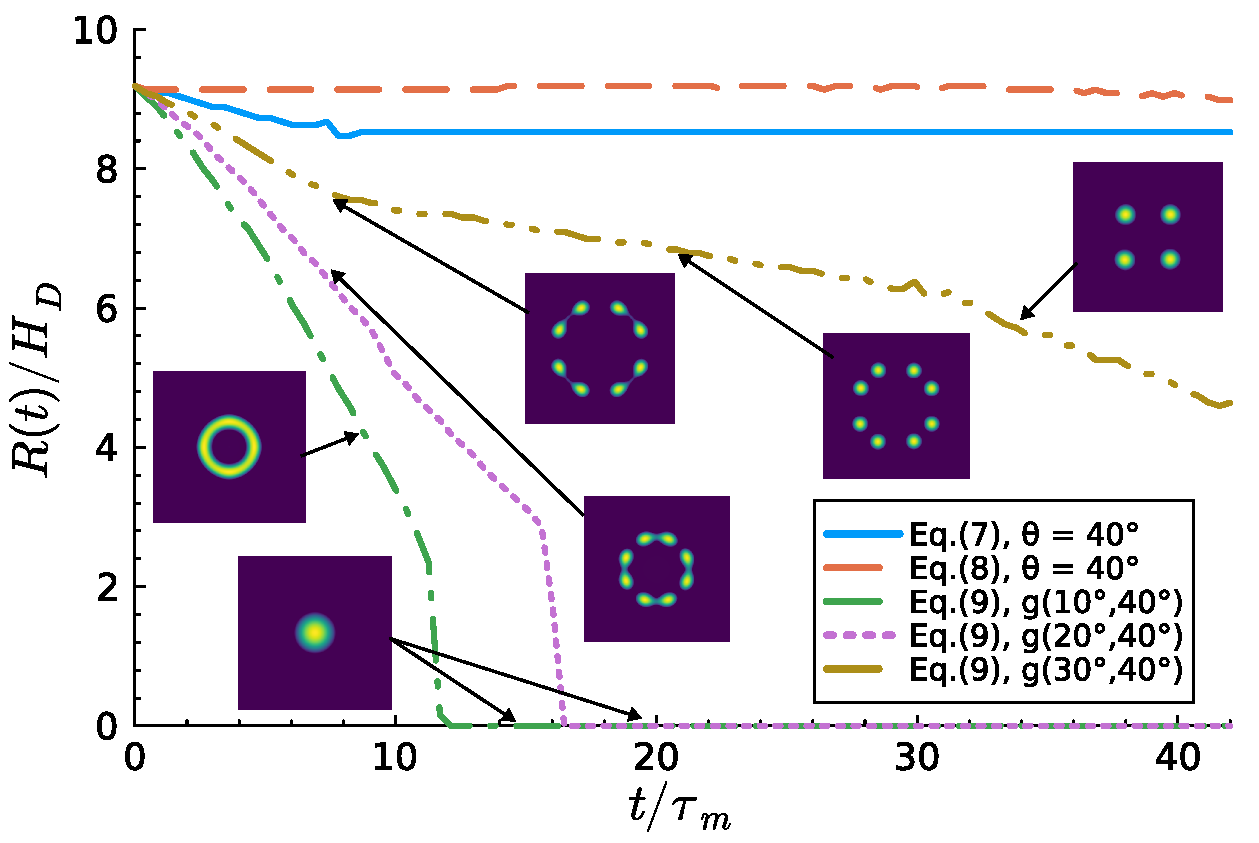
\includegraphics[width=0.48\textwidth]{assets/grad_heatmap.pdf}
    \caption{Evolution of the radius of a ring-rivulet $R(t)$ normalized by the droplet height $H_D$ for different contact angle cases (line styles and colours) and $\psi = 0.133$.
    The first argument of $g(a,b)$ is the contact angle in the centre of the numerical domain and the second argument is the contact angle at $R_0$ and beyond. 
    Besides the lines we add heatmap snapshots of the film thickness $h(\mathbf{x},t)$ where yellow indicates a large value and dark blue a small value (colorbars are not scaled).}
    \label{fig:negativewetgrad}
\end{figure}
As the last part of this section we want to address the impact of a linear wettability gradient on the dynamics of the ring-rivulet. 
We first consider a positive wettability gradient, thus the wettability increases towards the centre of the domain starting from $R_0$ and is kept constant for $\xi > R_0$.
Fig.~\ref{fig:negativewetgrad} shows measurements of the ring radius $R(t)$ for different wettability scenarios with $\psi_0 = 0.133$.
The different colours depict different simulations, including the uniform substrate and the banded pattern shown in blue and orange respectively.
These two line show only a minor change in $R(t)$ and then appear to be stationary.
Which can be explained by the fact that the ring ruptures and forms droplets, these droplets do not move and therefore $R(t)$ does not change.
On the other hand the remaining three curves show the impact of a wettability gradient.  
In green we have the highest wettability gradient, starting from $\theta = 40^{\circ}$ at $\xi = R_0$ decreasing to $\theta = 10^{\circ}$ at $\xi = 0$. 
The dynamical evolution of the ring-rivulet is clearly different from the uniform and banded case.
Instead of a breakup we see a constant contraction and the ring remains stable until a single droplet is formed at the centre of the substrate.
While the radius of that droplet is not zero we made the arbitrary choice to set $R(t) = 0$ if the liquid-solid area is a disk, inline with the topological change and the switch of the Euler characteristic $\chi$ from 0 to 1.
We see that a wettability gradient can transform an initial condition that would break up into a collapsing one.

Even more interesting are the two remaining curves, thus the purple and golden one.
From green to golden the wettability gradient becomes smaller, going from a $30^{\circ}$ difference to a $10^{\circ}$ difference.
The purple is in between the green and the golden with a $20^{\circ}$ difference. 
Similar to the green one we see a linear change in $R(t)$ with a kink shortly before a single droplet is formed.
However, in this case the ring-rivulet is breaking up and forms four intermediate droplets, as shown with heatmaps in Fig.~\ref{fig:negativewetgrad}.
Due to the wettability gradient these droplets are not stationary, but are advected towards the centre of the substrate and form a single droplet on a slightly longer time scale as compared to the green curve.
The golden curve has the smallest wettability gradient which effectively deceleration the dynamics.
Similar to the purple one the rivulet breaks up, but it forms eight droplets instead of four, similar to the uniform substrate.
Again the droplets are advected towards the centre of the substrate, but as the gradient is smaller the radius changes on longer time scales. 
Around $t\approx 32\tau_m$ the two droplets closest to each other coalesce and after $t\approx 35\tau_m$ we only have four droplets.
The final state again would be a single droplet in the centre of the substrate.

\begin{figure}
    \centering
    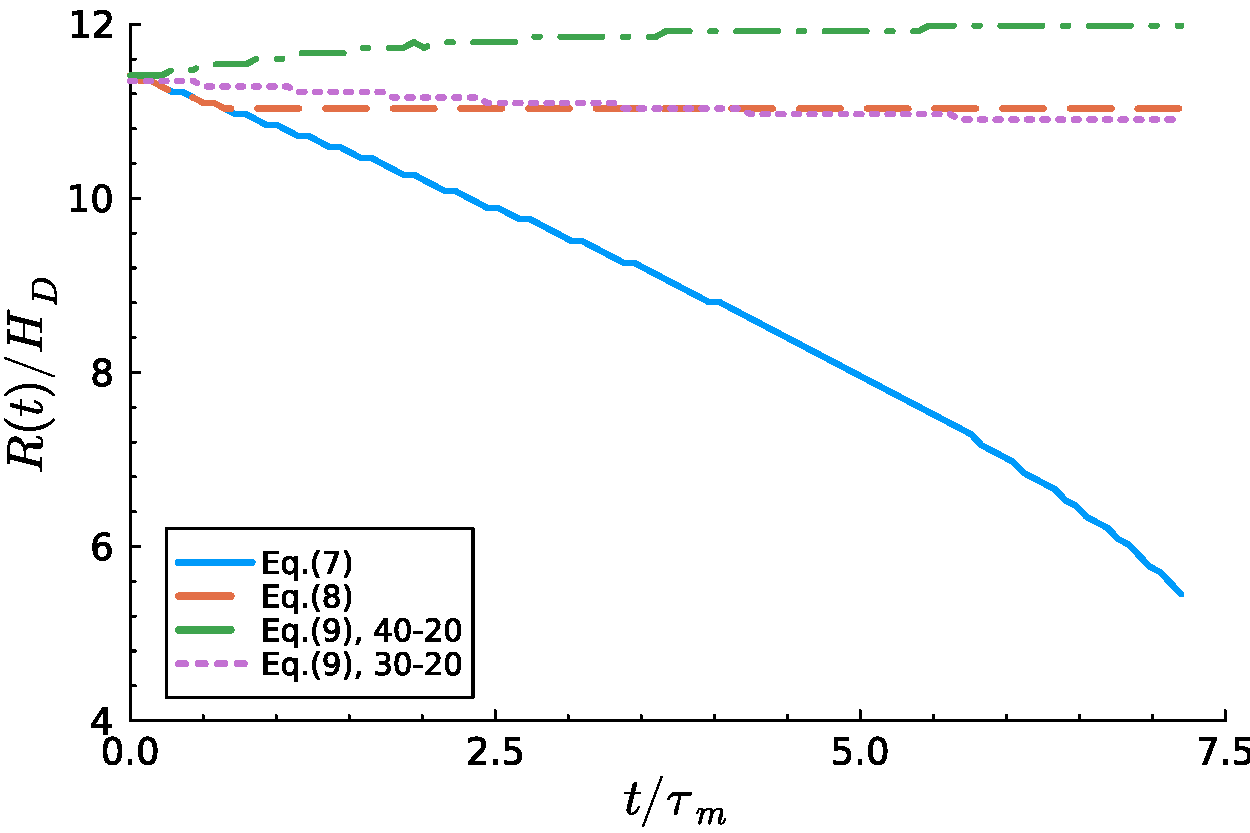
\includegraphics[width=0.48\textwidth]{assets/radius_time_gradient_positive.pdf}
    \caption{Evolution of the radius of a ring-rivulet $R(t)$ normalized by the droplet height $H_D$ for different contact angle cases (line styles and colours) and $\psi = 0.3$.
    The first argument of $g(a,b)$ is the contact angle in the centre of the numerical domain and the second argument is the contact angle at $R_0$ and beyond.}
    \label{fig:positivewetgrad}
\end{figure}
A wettability gradient, therefore, allows us to alter the time scales $t_b$ and $t_c$.
For the smallest positive gradient, the golden curve, we are in fact able to switch between an eight, four and one droplet state simply be means of the radial gradient. 
For completeness we then performed numerical experiments with a negative wettability gradient, thus the centre of the substrate is less wettable than the rest.
In Fig.~\ref{fig:positivewetgrad} we show $R(t)$ data of four simulations with $\psi_0 = 0.3$.
The blue curve depicts the evolution on the uniform substrate, as indicated in Fig.~\ref{fig:max_drops} $\psi_0$ values larger than $0.25$ lead to a collapse.
Unsurprisingly, the banded pattern prohibits this collapse and stabilizes the ring during the duration of the numerical experiment as shown by the orange dashed line.
Additionally we have two negative gradients shown in green and purple. 
The larger negative gradient, the green curve, the centre of the rivulet is actually pushed away from $R_0$ leading to an increase of radius.
Here we also observe a break up in the long time limit, due to the use of periodic boundary conditions we observe the coalescence of two droplets and thus only have three droplets.
Without periodic boundary conditions we most likely find four droplets which would agree with Eq.~(\ref{eq:maxDrops}).
For the smaller negative gradient we do not observe such an effect and the data is barely distinguishable from the banded case.
In neither of these two case we see a break up until the last iteration of our simulation.
However, once again a wettability gradient changes a collapsing state into a non collapsing one.

\section{Conclusions}\label{sec:conclu}
We have presented numerical experiments of a liquid ring-rivulet on a uniform and patterned substrate. 
The basis of our experiments is the thin film equation with a disjoining pressure model.
We are able to reproduce results of Gonz{\'a}lez et al.~\cite{gonzalezStabilityLiquidRing2013} and show some agreement for small $\psi_0$ values concerning the most unstable mode and as such the number of droplets, for both the uniform and a patterned substrate.
For $\psi_0 > 0.25$ the capillary retraction outpaces the breakup and the collapse is the more likely outcome.
We further found a good analytical approximation for the growth rate on the uniform substrate as shown in Fig.~\ref{fig:first_growth}. 

Our main aim, however, is to address the impact of wettability on the dynamics of the ring-rivulet.
We therefore considered two patterns, one that restricts the rivulet to a band and effectively removes the collapse mode and a positive as well as a negative wettability gradient towards the centre.
The banded pattern shows good agreement with the predicted number of droplets, in the small $\psi_0$ regime. 
Interestingly, the rupture times seems linearly correlated with $\psi_0$ as shown in Fig.~\ref{fig:bandBreakupT}.

The wettability gradient patterns on the other hand allow us to tune the two competing time scales, namely the breakup time $t_b$ and the collapse time $t_c$.
We show this in Fig.~\ref{fig:negativewetgrad}, where the initial conditions ($\psi \approx 0.13$) favor a breakup of the ring, or $t_b < t_c$.
By applying the positive wettability gradient we can not only force the rivulet to end up in a collapsed state, but can approach this state via different trajectories. 
Having a strong radial gradient allows to skip the breakup and thus $t_c < t_b$.
If we however the gradient we can pass by different droplet states with either four or eight droplets.
In case of a negative radial wettability gradient we find that similar to the band pattern, collapse is unlikely.

As a future perspective of this work we would like to add thermal fluctuations to the system as some experimental realizations using molten metal.
On the other hand a dynamic pattern may allow for radial breakup as well, because currently we only observed azimuthal breakup.

\section*{Author Contributions}
We strongly encourage authors to include author contributions and recommend using \href{https://casrai.org/credit/}{CRediT} for standardised contribution descriptions. Please refer to our general \href{https://www.rsc.org/journals-books-databases/journal-authors-reviewers/author-responsibilities/}{author guidelines} for more information about authorship.

For footnotes in the main text of the article please number the footnotes to avoid duplicate symbols. \textit{e.g.}\ \texttt{\textbackslash footnote[num]\{your text\}}. The corresponding author $\ast$ counts as footnote 1, ESI as footnote 2, \textit{e.g.}\ if there is no ESI, please start at [num]=[2], if ESI is cited in the title please start at [num]=[3] \textit{etc.} Please also cite the ESI within the main body of the text using \dag. For the reference section, the style file \texttt{rsc.bst} can be used to generate the correct reference style.

\section*{Conflicts of interest}
There are no conflicts to declare.

\section*{Acknowledgements}
S. Z. and J. R. acknowledge the financial support from the Independent Research Fund Denmark through a DFF Sapere Aude Research Leader grant (grant number 9063-00018B).



%%%END OF MAIN TEXT%%%

%The \balance command can be used to balance the columns on the final page if desired. It should be placed anywhere within the first column of the last page.

\balance

%If notes are included in your references you can change the title from 'References' to 'Notes and references' using the following command:
%\renewcommand\refname{Notes and references}

%%%REFERENCES%%%
\bibliography{rsc} %You need to replace "rsc" on this line with the name of your .bib file
\bibliographystyle{rsc} %the RSC's .bst file

\appendix
\section{Numerical model and parameters}\label{app:numerics}
The numerical model is based on a single relaxation (SRT) time lattice Boltzmann method. 
The relaxation time $\tau$ is set to $\tau = 1$ in all our numerical experiments. 
This means that the fluid's kinematic viscosity $\nu$ is set to $\nu = 1/6$ and kept constant for all simulations.  


The surface tension $\gamma$ is set to $\gamma = 10^{-2}$ for all results presented here.
We did in fact simulate with different values of $\gamma$ but found that the effect is an overall rescaling of the time scale, larger $\gamma$ speeds up all dynamics, lower $\gamma$ values slows them down.

Lastly $\alpha_{\delta}(h)$ is a substrate friction term that mimics a slip boundary condition with an effective slip length $\delta$
\begin{equation}\label{eq:alphafric_app}
\alpha_{\delta}(h) = \frac{6h}{(2 h^2 + 6 \delta h + 3 \delta^2)}.
\end{equation}
By introducing a precursor layer $h_{\ast}$ and a slip length $\delta$ we regularize the contact line divergence~\cite{huhHydrodynamicModelSteady1971}. 
The slip length lies within the weak/intermediate slip regime~\cite{peschkaSignaturesSlipDewetting2019,fetzerQuantifyingHydrodynamicSlip2007, munchLubricationModelsSmall2005} and the thickness of the precursor film is set to $h_{\ast} = 0.05$.

By applying this solution for $\mathbf{u}$ to the continuity equation we have
\begin{equation}\label{eq:thinsolve_app}
     \partial_t h(\mathbf{x},t) = \nabla\cdot\left(M_{\delta}(h)\nabla p_{\mbox{\tiny{film}}}\right),
\end{equation}
with the mobility function $M_{\delta}(h) = \frac{h^2}{\mu\alpha_{\delta}(h)}$ which for the no-slip boundary condition $(\delta \rightarrow 0)$ reduces to $M_{0}(h) = h^3/3\mu$.
Without loss of generality we set $\rho_0 = 1$ and thus the dynamic viscosity is $\mu = \rho_0 \nu = 1/6$. 

The numerical domain consists of a square lattice with $512\Delta x$ in both horizontal directions.
We further use biperiodic boundary conditions at the edges of the domain. 





\end{document}
